\documentclass[handout, 10pt]{beamer}

%\usepackage[backend=bibtex,firstinits=true,style=verbose-inote,citestyle=authortitle]{biblatex}
\usepackage{bm}
\usepackage{graphicx}
\usepackage{subcaption}
\usepackage{amsmath}
\usepackage{amsfonts}
\usepackage{makecell}
\usepackage{filecontents}
\usepackage{biblatex}
% \newcommand{\expect}[2][]{
\ifthenelse{\equal{#1}{}}{
\mathbb{E}\left[#2\right]
}{
\underset{#1}{\mathbb{E}}\left[#2\right]
}}

\newcommand{\cov}[2][]{
\ifthenelse{\equal{#1}{}}{
\text{Cov}\left[#2\right]
}{
\underset{#1}{\text{Cov}}\left[#2\right]
}}


\newcommand{\var}[2][]{
\ifthenelse{\equal{#1}{}}{
\text{Var}[#2]
}{
\underset{#1}{\text{Var}}[#2]
}}

\newcommand{\loss}[2][]{
\ifthenelse{\equal{#1}{}}{
\mathcal{L}(#2)
}{
\mathcal{L}_{#1}(#2)
}}

\newcommand{\kl}[2]{
\text{D}_\text{KL}[#1 \parallel #2]
}

\newcommand{\R}{\mathbb{R}}
%\newcommand{\Prob}{\mathbb{P}}

\newcommand{\1}[1]{\mathds{1}\{#1\}}


%\usecolortheme{dolphin}
\setbeamertemplate{navigation symbols}{}
\setbeamertemplate{section in toc}{\inserttocsectionnumber.~\inserttocsection}

\begin{filecontents*}{references.bib}
@incollection{WANN,
title = {Weight Agnostic Neural Networks},
author = {Gaier, Adam and Ha, David},
booktitle = {Advances in Neural Information Processing Systems 32},
editor = {H. Wallach and H. Larochelle and A. Beygelzimer and F. d\textquotesingle Alch\'{e}-Buc and E. Fox and R. Garnett},
pages = {5364--5378},
year = {2019},
publisher = {Curran Associates, Inc.},
url = {http://papers.nips.cc/paper/8777-weight-agnostic-neural-networks.pdf}
}
\end{filecontents*}

\addbibresource{references.bib}


\title{Genome Bottleneck in Deep Learning}
%\subtitle{}
\author{Ivan Skorokhodov}
%\date{}
%\logo{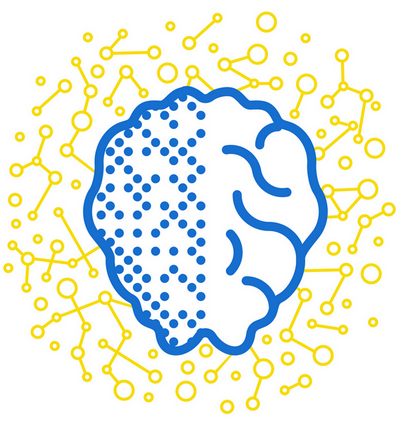
\includegraphics[height=1cm]{images/ipavlov-logo.png}}

\newcommand{\citepaper}[1]{\citetitle{#1} by \citeauthor{#1}}

%\graphicspath{{./images}}

%\usetheme{lucid}
\begin{document}

\begin{frame}
    \titlepage
\end{frame}

\begin{frame}{Overview}
    \begin{itemize}
        \item\pause Animals and humans have a lot of innate abilities and inclinations:
            \begin{itemize}
                \item\pause A colt can walk within hours after birth
                \item\pause Turkeys can visually recognize predators shortly after hatching
                \item\pause Sharks are attracted to blood immediately after birth
                \item\pause Spiders are born ready to hunt
                \item\pause Human newborns can recognize human faces% (which they prefer over other objects), and can even discriminate between happy and sad expressions
            \end{itemize}
        \item\pause I.e. they have higher than random performance at initialization and good few-shot learning capabilities for critical tasks
        \item\pause At birth, an infant has $\approx 86$ billion neurons (this number remains almost the same during life) and 10-100 trillion synapses which grow rapidly over the first 3 years \footnote{http://www.urbanchildinstitute.org/why-0-3/baby-and-brain}.
%        \item\pause Human brain consists on 90 billion neurons and 150 trillion synapses
        \begin{itemize}
            \item\pause Even if each value is binary it is $\approx 1300$ GB of information
        \end{itemize}
        \item\pause Human genome can store up to 800 MB of data, which is 1625 times less than amount of information in an infant brain\footnote{if all the genome stores is an information about the brain}
        \item\pause So, human genome cannot store all the information about the brain
        \item\pause How then genome can encode so strong?
    \end{itemize}
\end{frame}

\end{document}
